\documentclass[11pt,letterpaper,twocolumn]{article}

\usepackage[utf8]{inputenc}
\usepackage[portuguese]{babel}
\usepackage{float}
\usepackage{xcolor}
\usepackage{verbatim}
\usepackage{charter}
\usepackage{amsmath}
\usepackage{appendix}
\usepackage{ragged2e}
\usepackage{array}
\usepackage{etoolbox}
\usepackage{fancyhdr}
\usepackage{booktabs}
\usepackage{arydshln}
\usepackage{caption}
\usepackage{subcaption}
\usepackage{enumitem}
\usepackage[bottom=3 cm,top=2.0cm,left=2.0cm,right=2.0cm]{geometry}
\usepackage{graphicx}
\usepackage{mathtools}
\usepackage{multirow}
\usepackage{pdfpages}
\usepackage{subfiles}
\usepackage[compact]{titlesec}
\usepackage{stfloats}
\usepackage{hyperref}
\usepackage{amsfonts}
\usepackage[export]{adjustbox}


\setlength{\columnsep}{30pt}

%\titlelabel{\thetitle.\quad}

\pagestyle{fancy}
\fancyhf{}
      
\fancyfoot{}
\fancyfoot[C]{\thepage} % page
\renewcommand{\headrulewidth}{0mm} % headrule width
\renewcommand{\footrulewidth}{0mm} % footrule width

\makeatletter
\patchcmd{\headrule}{\hrule}{\color{black}\hrule}{}{} % headrule
\patchcmd{\footrule}{\hrule}{\color{black}\hrule}{}{} % footrule
\makeatother

\definecolor{blueM}{cmyk}{1.0,0.49,0.0,0.47}
    
\begin{document}
\twocolumn[\begin{@twocolumnfalse}

\begin{minipage}{\textwidth}
\vspace{5mm}
    \Large{\textbf{Aplicação do MCMC na Modelagem dos Gols dos Campeonatos da CBF de 2013 a 2020}} 
    \vspace{3mm}
    
    \large{\textbf{Igor Patrício Michels}} 
    \vspace{2mm}\newline

    \fontsize{0.35cm}{0.5cm}\selectfont \textit{Escola de Matemática Aplicada, EMAp/FGV\newline 
    Rio de Janeiro/RJ, Brasil}
    \vspace{1mm} 
    
    \today

\end{minipage}

\small
\vspace{11pt}
\centerline{\rule{0.95\textwidth}{0.4pt}}

\begin{center}
    \begin{minipage}{0.9\textwidth}
        \noindent \textbf{Resumo:} 
        Esse trabalho tem como objetivo descrever a modelagem de gols por jogo nos campeonatos realizados pela CBF no período de 2013 a 2020 por meio da utilização de Cadeias de Markov Monte Carlo para a estimação de parâmetros. Dois modelos são propostos, um com uma Distribuição de Poisson e outro com uma Distribuição Gamma adaptada.
        \vspace{4mm}
        
        \noindent \textbf{Palavras chave:} MCMC, Método Iterativo, Modelagens de Gols, Distribuição de Poisson.
    \end{minipage}
\end{center}

\centerline{\rule{0.95\textwidth}{0.4pt}}

\vspace{15pt}
\end{@twocolumnfalse}]

\section{Introdução}
\justify

Em grandes competições esportivas sempre ocorrem especulações sobre o resultado de uma prova, jogo ou da própria competição. Essas especulações se intensificam em épocas de Copa do Mundo, principalmente com a mídia trazendo animais ``oráculos'', os quais prevem os resultados de algumas partidas, como o polvo Paul, na Copa do Mundo de 2010, e o gato Aquiles, da Copa do Mundo de 2018. Matematicamente, a modelagem esportiva tem aplicações práticas para jogos de azar, melhoria nas técnicas de coaching para motivar equipes ou jogadores, no jornalismo e nos próprios clubes com o intuito de melhorar o desempenho dos seus jogadores e de prevenir lesões, além de estudar o desempenho de seus rivais, podendo elaborar uma estratégia ótima para enfrentar os mesmos.

Nesse sentido, estudos relacionados aos resultados esportivos são cada vez mais frequentes, uma vez que buscam explicar o poder ofensivo e defensivo dos clubes, sendo a modelagem global dos dados, isto é, modelar o esporte como um todo ao invés de modelar uma competição ou os clubes dentro da mesma, um passo inicial para esse estudo.

Outro fator relevante é o modelo e a técnica utilizada para realizar a modelagem. Nesse trabalho, será proposto um modelo se valendo da Distribuição de Poisson, a qual é defendida na literatura para modelar a quantidade de gols em uma partida em virtude da ideia de que os gols são eventos independentes, bem como o resultado de duas partidas distintas. Uma abordagem secundária se dará pela Distribuição Gamma com certas adaptações. Já técnica utilizada nesse trabalho será a estimação por meio de Cadeias de Markov Monte Carlo (MCMC).

% Dessa forma, o presente estudo visa modelar a quantidade de gols em uma partida das competições da CBF, isso é, da Copa do Brasil e dos Campeonatos Brasileiros da Série A até a Série D com duas modelagens distintas implementadas via MCMC: a modelagem pela distribuição de Poisson e a modelagem pela distribuição Gamma. Como resultado lateral, poder-se-á ter um melhor entendimento das Cadeias de Markov Monte Carlo no processo de cálculo de uma posteriori.

\section{Metodologia}
\justify

Conforme citado anteriormente, o objetivo desse estudo é modelar a quantidade de gols em uma partida das competições da CBF. Para isso, os dados utilizados foram coletados diretamente do site da CBF por meio das súmulas das partidas em um trabalho anterior \cite{partidas}, com tratamento realizado via Python. As simulações foram realizadas por meio da mesma linguagem com a implementação do MCMC de maneira similar a vista em \cite{mcmc}.

A modelagem foi realizada tanto globalmente quanto individualmente a nível de competição, isto é, foram analisados tanto os dados dos jogos como um todo, juntando todos os jogos de todas as competições, quanto os jogos de uma competição específica, como apenas os jogos da Série A, por exemplo. Entretanto, nesse trabalho será discutido apenas os resultados da questão global, os gráficos desenvolvidos pela análise de uma competição específica podem ser vistos em \cite{trabalho}.

A escolha pela linguagem Python se deve pela facilidade na implementação e execução do MCMC, bem como para a geração dos gráficos, ambas tarefas realizadas com utilização das ferramentas oriundas dos pacotes {\fontfamily{pcr}\selectfont Numpy}, {\fontfamily{pcr}\selectfont Matplotlib}, {\fontfamily{pcr}\selectfont Statistics} e {\fontfamily{pcr}\selectfont Scipy}.

\section{Markov Chain Monte Carlo}

Nessa seção iremos abordar a modelagem das Cadeias de Markov Monte Carlo no contexto das distribuições Poisson e Gamma de modo a encontrar uma distribuição a posteriori que busque explicar os dados observados. A escolha da distribuição de Poisson se dá pelo fato da mesma ser discreta e não negativa, assim como o fenômeno que estamos modelando. Já a Gamma foi escolhida como distribuição alternativa, uma vez que a mesma é contínua e estritamente positiva, pela qual é possível comparar o desempenho do MCMC com relação a outra distribuição de probabilidade. 

\subsection{Modelagem com a Poisson}
\label{poisson}
\justify

Podemos iniciar a modelagem vendo os dados que dispomos. Dessa forma, analisando a quantidade de gols por partida nas competições da CBF de 2013 a 2020 temos o dado observado na Figura \ref{fig01p}.
\begin{figure}[hbt]
    \centering
    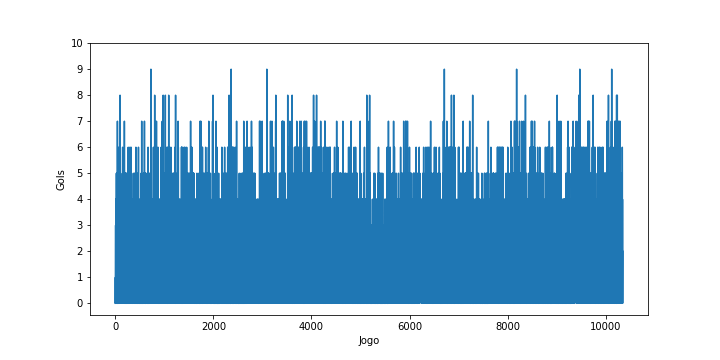
\includegraphics[scale = 0.40, center]{Poisson/fig01 - poisson.png}
    \caption{Gols por jogo no período de 2013 a 2020 nas competições da CBF.}
    \label{fig01p}
\end{figure}

% A análise dos dados conforme a Figura \ref{fig01p} mostra que a quantidade de gols é nula em uma grande quantidade consecutiva de jogos. Esse problema se deu em virtude de que alguns jogos não foram encontrados durante a coleta de jogos. Além disso, os gols de algumas partidas não foram encontrados. A inclusão de tais jogos no modelo se dará por dois motivos. O primeiro pelo fato de não haver uma diferenciação clara entre jogos que resultaram em zero a zero e jogos que não foram encontrados ou cujos gols não foram encontrados e também com o intuito de considerar um ruído nos dados, isto é, analisar o comportamento do MCMC quando existe ruído nos dados

Da forma como os dados estão expostos é difícil fazer qualquer análise sobre sua distribuição. Dessa forma, ao trazer os mesmos dados, mas em forma de histograma, pode-se ter uma análise mais eficiente de como os mesmos se comportam. Assim, a Figura \ref{fig02p} traz a informação de quantos jogos possuem cada quantidade de gols nesse mesmo período.
\begin{figure}[hbt]
    \centering
    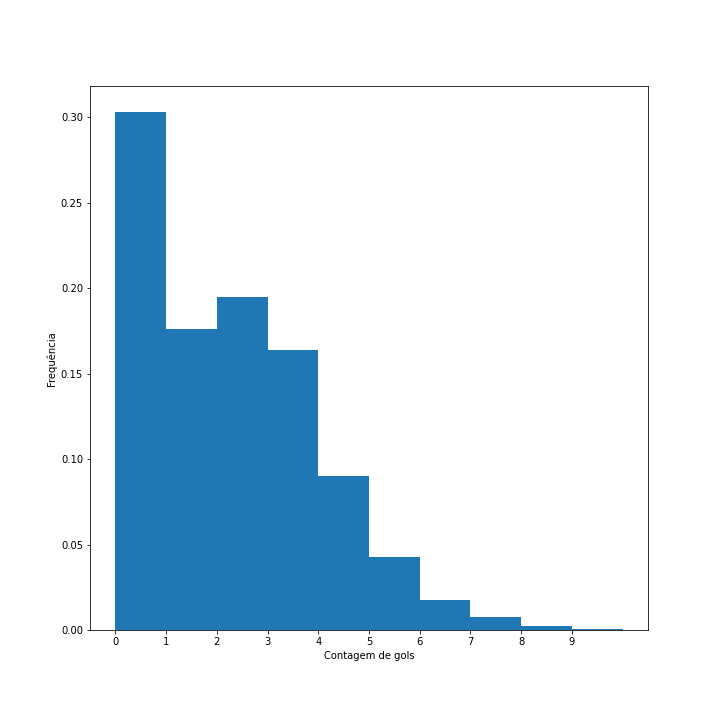
\includegraphics[scale = 0.40, center]{Poisson/fig02 - poisson.png}
    \caption{Histograma de jogos por quantidade de gols no período de 2013 a 2020 nas competições da CBF.}
    \label{fig02p}
\end{figure}

Pela Figura \ref{fig02p} pode-se observar uma certa similaridade dos dados com a Distribuição de Poisson para uma média $\lambda$. Esta similaridade não é uma mera coincidência, dado que podemos considerar independência entre os gols dentro de uma mesma partida e também independência entre as partidas, isto é, o resultado de um jogo não afeta o resultado de outro jogo. Dessa forma, a soma dos gols em uma partida também pode ser modelada como um processo de Poisson. Na literatura, pode-se citar \cite{poissoninan} e \cite{poissonmaher} como dois dos trabalhos que se valeram dessa abordagem para a modelagem de gols.

Tendo visto que faz sentido modelar a distribuição do gols por meio de uma Distribuição de Poisson, um estimador natural que surge para $\lambda$ se dá pelo Estimador de Máxima Verossimilhança, o qual muito utilizado na estatística frequentista. Dessa forma, pode-se estimar
\begin{equation}
    \lambda_{EMV} = \mu,
\end{equation}

\noindent sendo $\mu$ a média dos dados. Utilizando $\lambda_{EMV}$ como parâmetro da Poisson obtém-se a distribuição ilustrada na Figura \ref{fig04p}.
\begin{figure}[hbt]
    \centering
    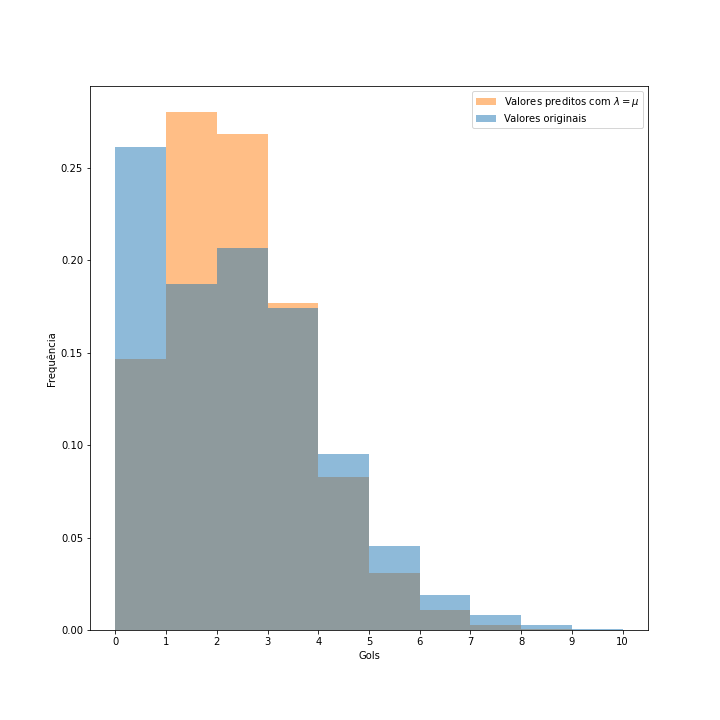
\includegraphics[scale = 0.40, center]{Poisson/fig04 - poisson.png}
    \caption{Distribuição obtida com $\lambda_{EMV}$.}
    \label{fig04p}
\end{figure}

Já a estimação se valendo do MCMC se dará por meio de um algoritmo iterativo. Para tanto, definem-se as seguintes funções:
\begin{itemize}
    \item
        uma função de transição de estados, isto é, uma função que recebe uma proposta atual $x$ para $\lambda$ e retorna uma proposta $x_n$ aleatória que, nesse estudo, se dá por $x_{n}\sim N(x, 0.5)$;
        
    \item
        uma função para calcular a log verossimilhança dos dados sob uma Distribuição de Poisso com parâmetro $\lambda$, a qual será representada por $L(\lambda)$;
        
    \item
        uma função de aceitação que calculará uma probabilidade $p$ que, nesse estudo, será dada por
        \begin{equation}
            p = 
            \left\{
                \begin{array}{rl}
                    1, & \text{se } L(x_n) > L(x) \\
                    \exp{\left(L(x_n) - L(x)\right)}, & \text{c.c.}
                \end{array}
            \right..
            \label{prob}
        \end{equation}
        Feito isso, aceita-se a proposta $x_n$ com probabilidade $p$.
\end{itemize}

Feitas tais definições, pode-se definir valor inicial para $x$ e, em cada iteração do algoritmo, o mesmo realizará o seguinte procedimento:
\begin{itemize}
    \item
        por meio da função de transição obtém-se $x_n$, uma nova proposta para $\lambda$;
        
    \item
        calcula-se $L(x)$ e $L\left(x_{n}\right)$;
        
    \item
        a função de aceitação verifica se aceita ou rejeita $x_n$;
        
    \item
        o valor de $x_n$ é armazenado numa lista de aceitos/rejeitados, conforme função de aceitação, bem como numa lista de propostas.
\end{itemize}

Como resultado, o algoritmo retornará as listas citadas na última parte da iteração, possibilitando analisar o comportamento do algoritmo durante suas iterações.

\subsection{Modelagem com a Gamma}
\label{gamma}
\justify

Primeiramente, conforme citado no início desta seção, temos que a Distribuição Gamma é contínua e estritamente positiva, indo contra os dados disponíveis, que são discretos (a quantidade de gols sempre é um número inteiro) e que podem ser nulos (pode ocorrer empate de zero a zero).

Dessa forma, uma maneira de utilizar a Gamma para modelar essa quantidade de gols se dá com alguns ajustes como, por exemplo, incrementar a quantidade de gols em $0.1$, fazendo com que os dados sejam estritamente positivos. Para resolver o problema da continuidade, pode-se analisar os valores à posteriori sob um histograma onde cada bin é o intervalo entre dois inteiros consecutivos ou, de forma equivalente, operar com o piso da distribuição.

Com esses ajustes, pode-se encontrar, de modo análogo a abordagem anterior, um estimador natural para a quantidade de gols. Isto é, por meio do Método dos Momentos, pode-se ver que
\begin{equation}
    \alpha = \dfrac{\mu^2}{\sigma^2}\text{ e } \beta = \dfrac{\mu}{\sigma^2},
    \label{momentos}
\end{equation}

\noindent sendo $\mu$ e $\sigma^2$ a média amostral e a variância amostral, respectivamente, apresentam uma boa estimativa para os parâmetros a serem procurados. A modelagem de uma Gamma com os parâmetros da Equação \ref{momentos} resulta no modelo da Figura \ref{fig04g}.
\begin{figure}[hbt]
    \centering
    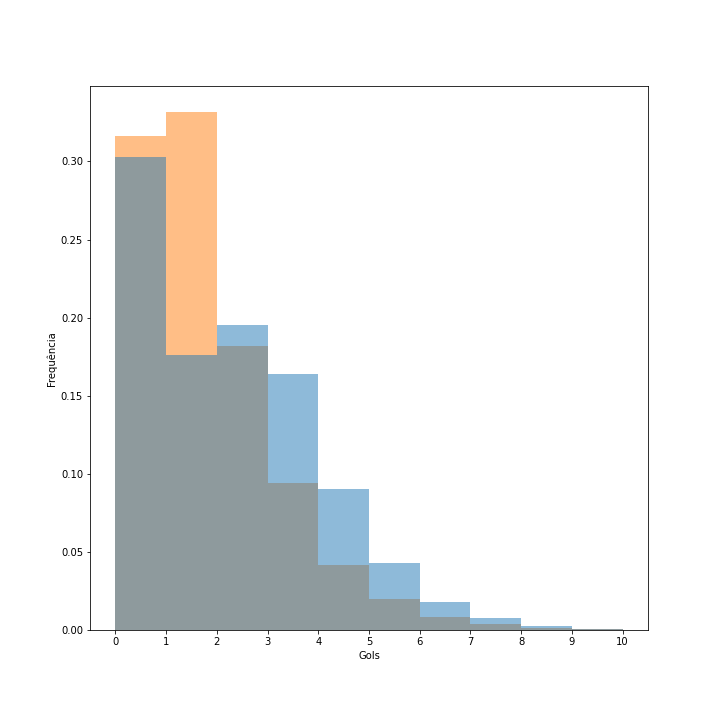
\includegraphics[scale = 0.40, center]{Gamma/fig04 - gamma.png}
    \caption{Distribuição obtida estimando $\alpha$ e $\beta$ pelo Método dos Momentos.}
    \label{fig04g}
\end{figure}

Já a modelagem pelo MCMC poderá ser realizada de modo similar ao realizado com a Distribuição de Poisson, isto é, por meio de um processo iterativo similar.

Dentre as funções definidas anteriormente, ocorre modificações na função de transição de estados, que, ao contrário da abordagem anterior onde retornava uma proposta escalar, passará a retornar um vetor $x_n = \left(\alpha_n, \beta_n\right)$ de modo que, nesse trabalho, $\alpha_{n}\sim N(\alpha, 0.05)$ e $\beta_{n}\sim N(\beta, 5)$. E a função de log verossimilhança é modificada de modo que calcula-se a log verossimilhança de uma Distribuição Gamma de parâmetros $x_p = \left(\alpha_p, \beta_p\right)$, retornando $L(x_p)$. A função de aceitação permanece a mesma, isto é, a probabilidade de aceitar uma proposta continua sendo expressa pela Equação \ref{prob}.

Definidas tais funções, pode-se definir os passos do algoritmo de modo análogo a modelagem com a Distribuição de Poisson.

\section{Resultados}
\justify

Nessa seção discutiremos alguns dos resultados observados durante a modelagem do fenômeno observado. Vale ressaltar que os dados observados contemplam todos os jogos de todas as competições da CBF, isto é, desde os jogos da Série A até os jogos da Série D e da Copa do Brasil. A quantidade de gols nos jogos observados irá variar conforme a competição. Por simplicidade, será aplicado o algoritmo sobre a distribuição ilustrada na Figura \ref{fig02p}, entretanto as mesmas ideias se aplicam para as demais competições. Os gráficos dispostos nesse documento, bem como os gráficos da modelagem das demais competições, podem ser encontrados em \cite{trabalho}.

\subsection{Distribuição de Poisson}
\justify

Aplicando a modelagem descrita na Seção \ref{poisson} obtém-se, com $\lambda_0 = 10$ e 50.000 iterações, uma sequência de propostas similares a ilustrada na imagem superior da Figura \ref{fig05p}. Já a imagem inferior destaca o caminho percorrido pelas propostas aceitas.
\begin{figure}[hbt]
    \centering
    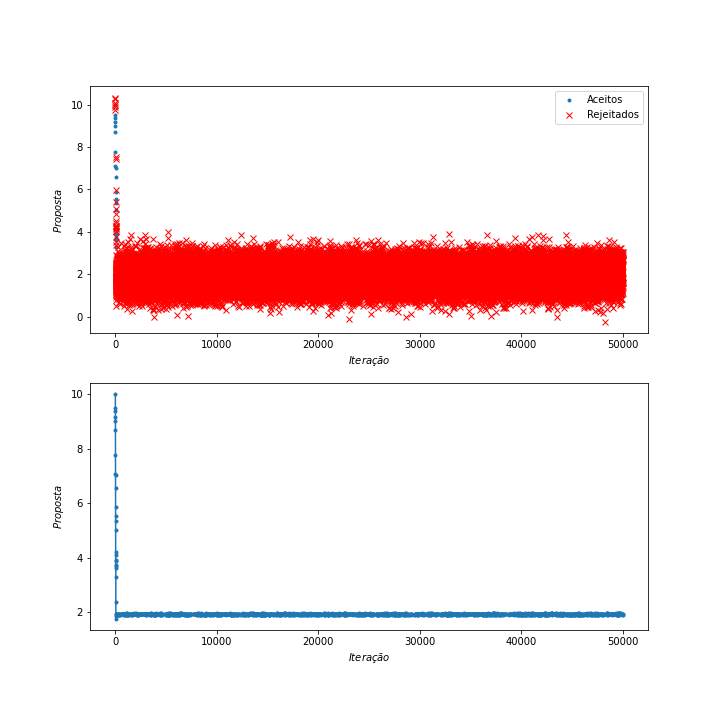
\includegraphics[scale = 0.40, center]{Poisson/fig05 - poisson.png}
    \caption{Na parte superior observam-se todas as propostas do algoritmo e na inferior o caminho percorrido pelas propostas aceitas.}
    \label{fig05p}
\end{figure}

Já a Figura \ref{fig06p} traz as mesmas informações que a Figura \ref{fig05p}, mas com um ``burn-in'' de 20\% das iterações com a intenção de retirar da visualização as discrepâncias geradas por uma priori não informativa.
\begin{figure}[hbt]
    \centering
    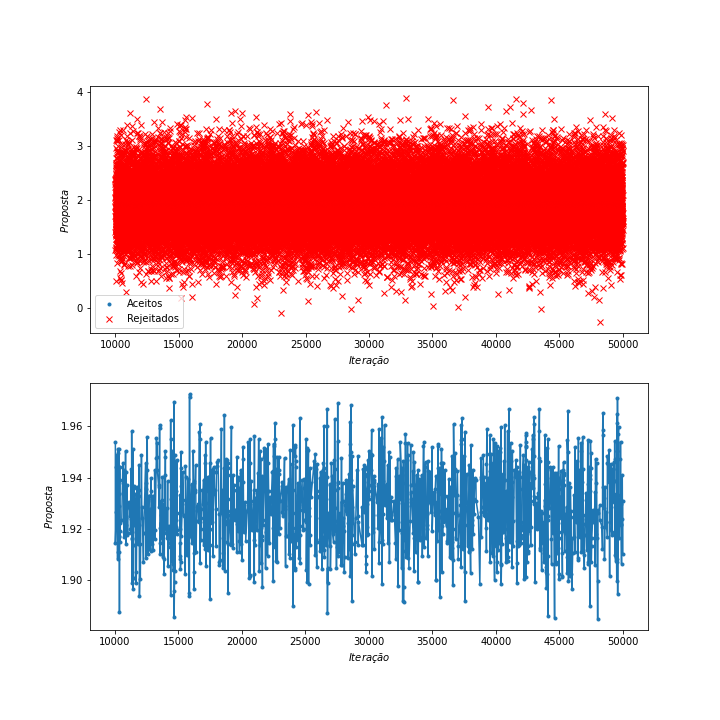
\includegraphics[scale = 0.40, center]{Poisson/fig06 - poisson.png}
    \caption{Na parte superior observam-se as últimas 40.000 propostas do algoritmo e na inferior o caminho percorrido pelas propostas aceitas dentre elas.}
    \label{fig06p}
\end{figure}

Tendo tais dados, pode-se analisar a região de aceitação para $\lambda$, isto é, a parte do espaço em que se concentram os valores para os quais a proposta $\lambda$ é aceita. Com essa ideia, pode-se observar na Figura \ref{fig07p} a região de aceitação de $\lambda$, bem como sua distribuição. Novamente, considera-se os dados com o ``burn-in''.
% \begin{figure*}[hbt]
%     \centering
%     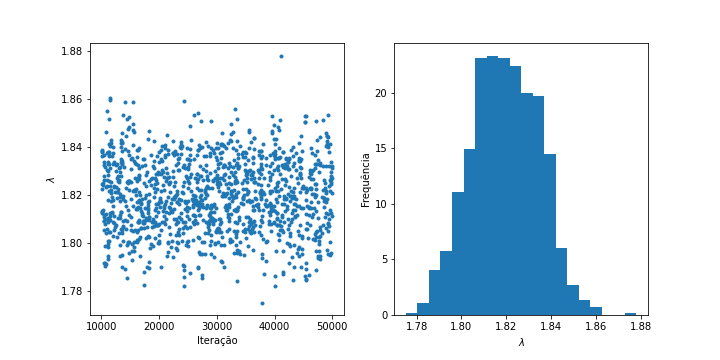
\includegraphics[scale = 0.7]{Poisson/fig07 - poisson.png}
%     \caption{À esquerda observa-se a região de aceitação de $\lambda$, enquanto à direita observa-se a distribuição do mesmo.}
%     \label{fig07p}
% \end{figure*}
\begin{figure}[hbt]
    \centering
    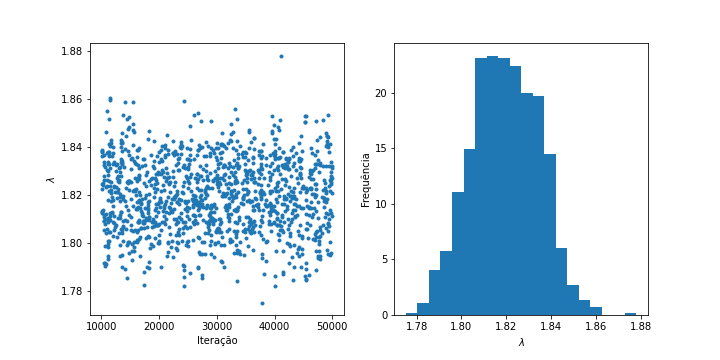
\includegraphics[scale = 0.40, center]{Poisson/fig07 - poisson.png}
    \caption{À esquerda observa-se a região de aceitação de $\lambda$, enquanto à direita observa-se a distribuição do mesmo.}
    \label{fig07p}
\end{figure}

Dessa forma, pode-se modelar o fenômeno observado tomando como $\lambda$ o valor médio das propostas aceitas. Com isso, obtém-se a distribuição à posteriori dos dados, conforme ilustrado na Figura \ref{fig08p}. A ideia de utilizar o valor médio se dá com o intuito de minimizar os efeitos gerados pela probabilidade de aceitar uma proposta caso o valor da log verossimilhança diminua.
\begin{figure}[hbt]
    \centering
    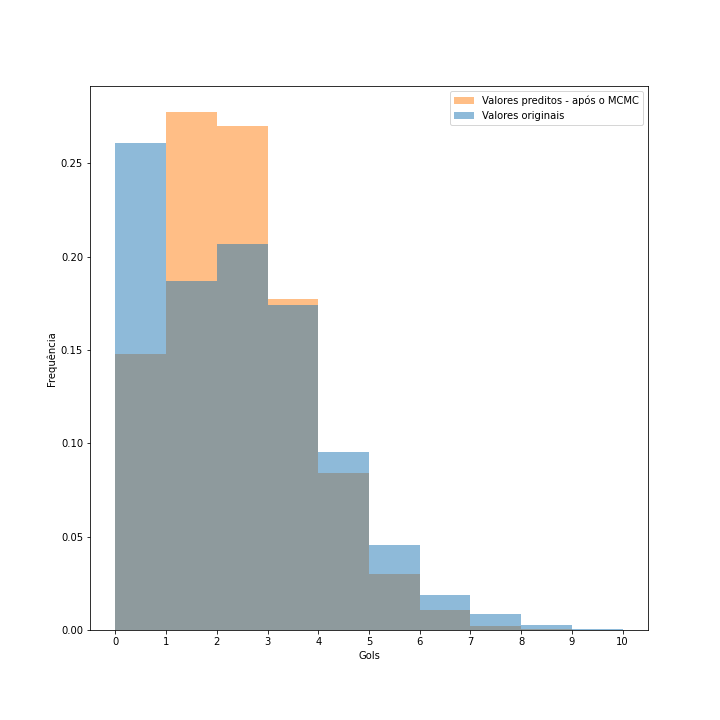
\includegraphics[scale = 0.40, center]{Poisson/fig08 - poisson.png}
    \caption{Distribuição a posteriori com distribuição de Poisson.}
    \label{fig08p}
\end{figure}

Comparando a posteriori com a estimativa obtida com $\lambda_{EMV}$, isto é, as distribuições das Figuras \ref{fig08p} e \ref{fig04p}, nota-se ambas parecem similares. Analisando o algoritmo utilizado pode-se perceber que isso é algo natural, uma vez que o algoritmo aceita uma sugestão $\lambda_n$ se a log verossimilhança aumenta ou, caso contrário, com uma probabilidade igual a razão entre a verossimilhança em $\lambda_n$ e $\lambda$.

\subsection{Distribuição Gamma}
\justify

Já a aplicação da modelagem com a Distribuição Gamma descrita na Seção \ref{gamma} requer um pouco mais de atenção, uma vez que a mesma é mais complexa por requerer dois parâmetros. Dessa forma, usando como parâmetros iniciais o vetor $x_0 = (1, 1)$, isto é, $\alpha_0 = \beta_0 = 1$, bem como 100.000 iterações e o incremento citado de 0.1 na quantidade de gols por jogo, pode-se aplicar o algoritmo, o qual irá fornecer dados com os quais geram-se observações similares as realizadas com a modelagem pela Distribuição de Poisson. Dessa forma, a Figura \ref{fig05g} ilustra os passos do algoritmo.
\begin{figure}[hbt]
    \centering
    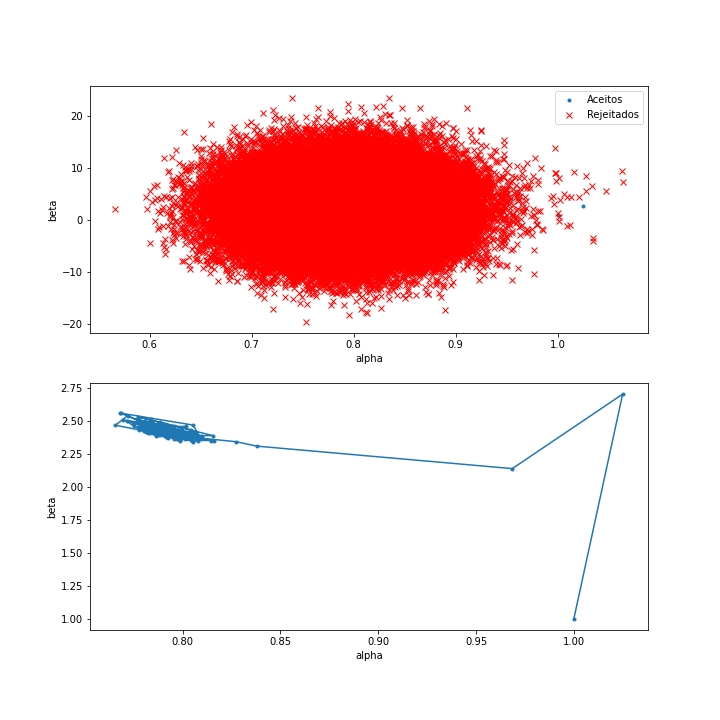
\includegraphics[scale = 0.40, center]{Gamma/fig05 - gamma.png}
    \caption{Na imagem superior observam-se todas as propostas do algoritmo e na inferior o caminho percorrido pelas propostas aceitas.}
    \label{fig05g}
\end{figure}

De maneira análoga a modelagem anterior, o ``burn-in'' dos 20\% primeiros passos poderá possibilitar uma análise mais concreta das iterações. Assim, a Figura \ref{fig06g} apresenta os últimos 80.000 passos do algoritmo.
\begin{figure}[hbt]
    \centering
    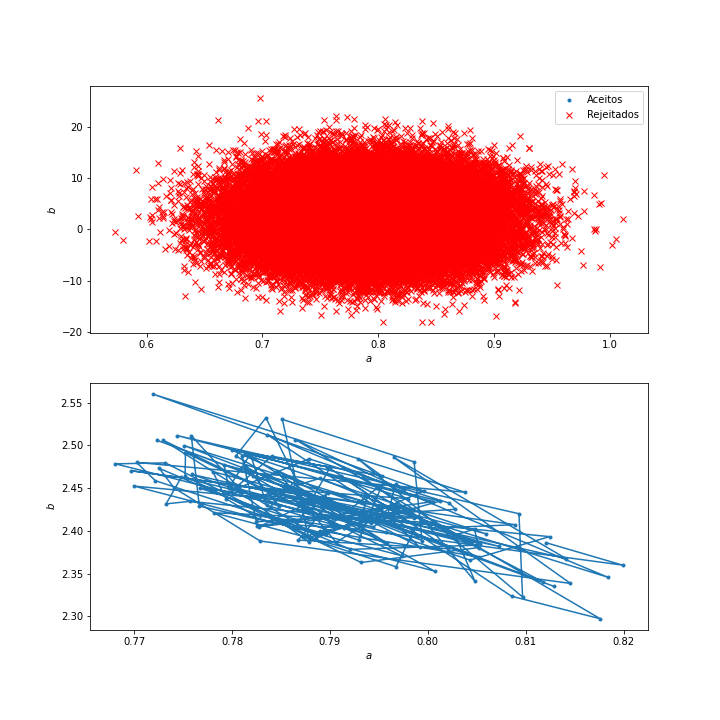
\includegraphics[scale = 0.40, center]{Gamma/fig06 - gamma.png}
    \caption{Na imagem superior observam-se as últimas 80.000 propostas do algoritmo e na inferior o caminho percorrido pelas propostas aceitas dentre elas.}
    \label{fig06g}
\end{figure}

A região de aceitação para uma proposta é um pouco mais complexa que no caso anterior, uma vez que $x\in \mathbb{R}^2$. Entretanto, por meio de um mapa de calor é possível visualizar a região de aceitação conjunta para $\alpha$ e $\beta$, conforme ilustrado na Figura \ref{fig09g}.
% podemos analisar as regiões de aceitação para cada coordenada independentemente, conforme visto nas Figuras \ref{fig07g} e \ref{fig08g}.
% \begin{figure*}[hbt]
%     \centering
%     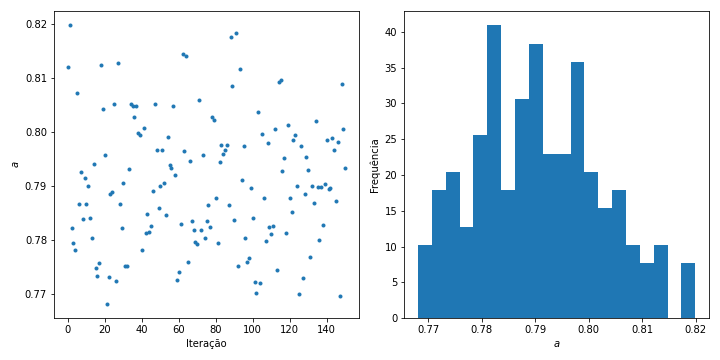
\includegraphics[scale = 0.7]{Gamma/fig07 - gamma.png}
%     \caption{À esquerda observa-se a região de aceitação de $\alpha$, enquanto à direita observa-se a distribuição do mesmo.}
%     \label{fig07g}
% \end{figure*}

% \begin{figure*}[hbt]
%     \centering
%     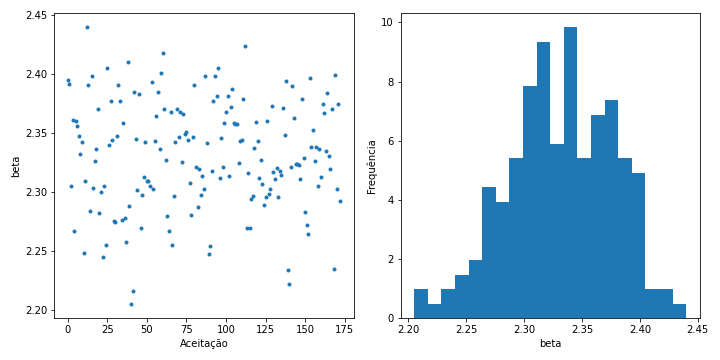
\includegraphics[scale = 0.7]{Gamma/fig08 - gamma.png}
%     \caption{À esquerda observa-se a região de aceitação de $\beta$, enquanto à direita observa-se a distribuição do mesmo.}
%     \label{fig08g}
% \end{figure*}


% \begin{figure}[hbt]
%     \centering
%     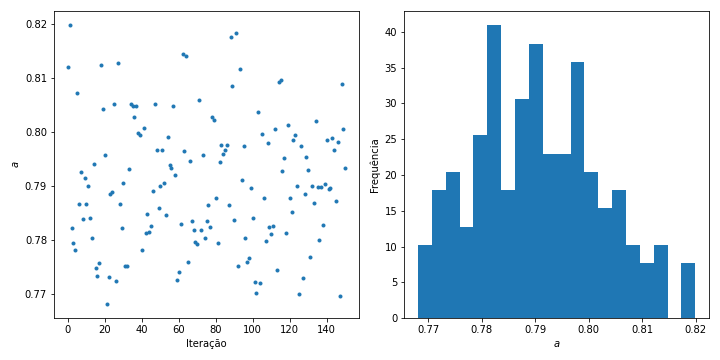
\includegraphics[scale = 0.40, center]{Gamma/fig07 - gamma.png}
%     \caption{À esquerda observa-se a região de aceitação de $\alpha$, enquanto à direita observa-se a distribuição do mesmo.}
%     \label{fig07g}
% \end{figure}

% \begin{figure}[hbt]
%     \centering
%     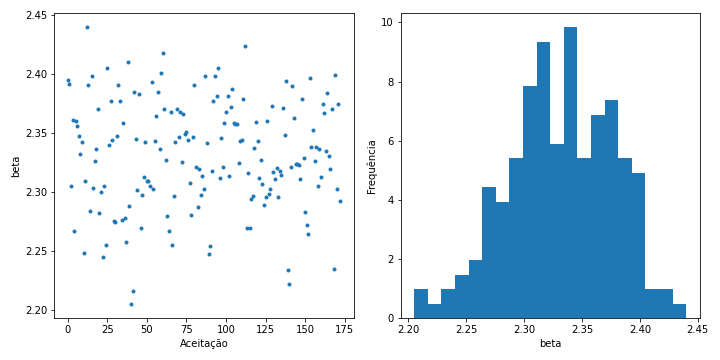
\includegraphics[scale = 0.40, center]{Gamma/fig08 - gamma.png}
%     \caption{À esquerda observa-se a região de aceitação de $\beta$, enquanto à direita observa-se a distribuição do mesmo.}
%     \label{fig08g}
% \end{figure}

% A região de aceitação conjunta para $\alpha$ e $\beta$ pode ser visualizada por meio de um mapa de calor, o qual é ilustrado na Figura \ref{fig09g}.
\begin{figure}[hbt]
    \centering
    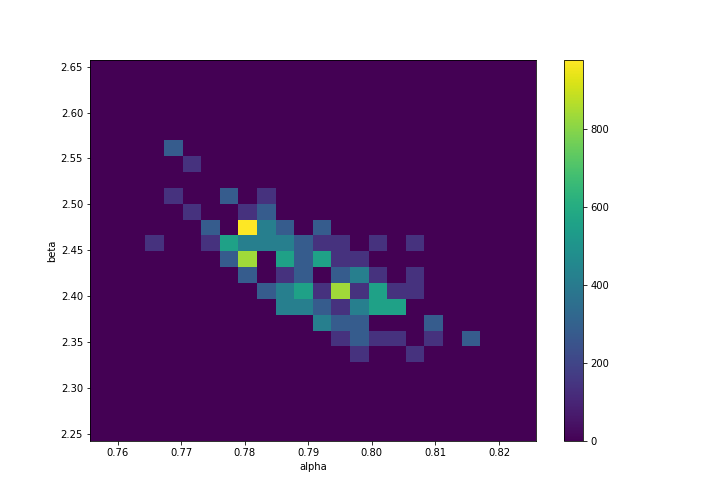
\includegraphics[scale = 0.40, center]{Gamma/fig09 - gamma.png}
    \caption{Região de aceitação conjunta de $\alpha$ e $\beta$.}
    \label{fig09g}
\end{figure}

Por fim, a distribuição à posteriori gerada pelo algoritmo aplicado a Distribuição Gamma pode ser dada por meio de uma Distribuição Gamma com parâmetros $\alpha = \mu_\alpha$ e $\beta = \mu_\beta$, onde $\mu_\alpha$ e $\mu_\beta$ representam, respectivamente, a média dos $\alpha$ e dos $\beta$ aceitos após aplicar o ``burn-in''. Novamente, a aplicação da média está relacionada com o intuito de minimizar os erros cometidos pelo fator aleatório na aceitação das propostas. A distribuição gerada por tais parâmetros pode ser encontrada na Figura \ref{fig10g}.
\begin{figure}[hbt]
    \centering
    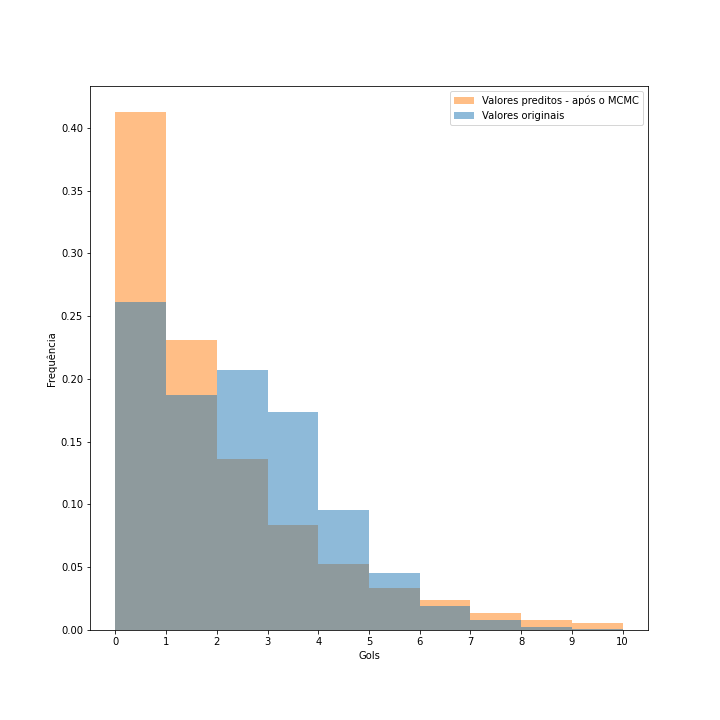
\includegraphics[scale = 0.40, center]{Gamma/fig10 - gamma.png}
    \caption{Distribuição à posteriori $Gamma(\mu_\alpha, \mu_\beta)$.}
    \label{fig10g}
\end{figure}

\section{Conclusão}
\justify

O modelo dado pela Distribuição de Poisson modela a maior parte dos jogos possuindo 1, 2 ou 3 gols, acertando grande parte dessas predições, mas errando uma parte considerável da mesmas. Além disso, o modelo também acaba errando, para baixo, a quantidade de de partidas que terminam com mais de 3 gols ou as em que não há gols. Boa parte desses erros é irrelevante, dado que a taxa de acerto é alta, entretanto, quando se trata de um placar com mais de 6 gols o modelo já não é totalmente capaz de prever.

Em contrapartida, a modelagem dada pela Distribuição Gamma já resulta em um modelo que contempla mais facilmente placares com muitos gols, inclusive superestimando as probabilidades desses placares. Além dos placares com muitos gols, essa modelagem superestima placares magros, como zero a zero ou um a zero, com o modelo dando uma probabilidade muito acima da frequência observada nos dados ao primeiro destes placares. Já os placares com quantidade de gols entre 2 e 5 são subestimados pelo modelo.

Comparativamente, ambos os modelos aparentam ter eficiência similar, se distinguindo apenas pelos pontos onde aparentam superestimar e subestimar os placares. Já levando em conta a eficiência do algoritmo, percebe-se que a modelagem pela Distribuição de Poisson é mais eficiente, uma vez que, por possuir apenas um parâmetro, apresenta bons resultados de convergência com menos iterações, enquanto o modelo com a Distribuição Gamma necessita de mais iterações para ter um resultado similar.

\newpage
\begin{thebibliography}{9}

\bibitem{poissoninan} Inan, T. (2020). Using poisson model for goal prediction in European football. \textit{Journal of Human Sport and Exercise, in press}. doi: \url{https://doi.org/10.14198/jhse.2021.164.16}.

\bibitem{poissonmaher} Maher, M. J. (1982). Modelling Association Football Scores.

\bibitem{mcmc} Moukarzel, J. (2019). Markov Chain Monte Carlo. \textit{MCMC}. \url{https://github.com/Joseph94m/MCMC}.

\bibitem{partidas} Michels, I. (2021). Brazilian Soccer. \textit{Brazilian Soccer}. \url{https://github.com/IgorMichels/Brazilian_Soccer}.

\bibitem{trabalho} Michels, I. (2021). Statistical Modeling. \textit{Statistical Modeling}. \url{https://github.com/IgorMichels/Statistical_Modeling}.

\end{thebibliography}

\end{document}
